\documentclass[11pt]{article}

\usepackage[margin=1in]{geometry}
\usepackage{graphicx}
\usepackage{amsmath}
\usepackage{amsfonts}
\usepackage{amssymb}
\usepackage{hyperref}
\usepackage{graphicx}
\usepackage{parskip}
\usepackage{booktabs}
\graphicspath{ {./images/} }

\title{Project 1 Report - ME155C/ECE147C}
\author{Cole Giusto, Raaghav Thirumaligai, Tien Nguyen}
\date{\today}

\begin{document}
\maketitle

% ---------------------------------------------------
% Abstract
% ---------------------------------------------------
\begin{abstract}
% [Report] Abstract:
% Summarize the content of the entire document in one or two paragraphs.
% Focus on key achievements.

In this project, we design a controller for a two mass - one spring, cart system. The goal is to optimize the performance of the second cart's response to a step input to the reference through control of the first cart's behavior, with respect to several key control metrics. We look at optimizing for a very short settling time along with minimizing the amount of overshoot. The 'undershoot' is treated as an acceptable behavior since the cart will pass through this region, so we give ourselves the difficulty of treating the overshoot as a highly undesirable set.
We achieve our goals with a settling time under three seconds along with less than one percent overshoot. 
% Example structure:
% - One paragraph explaining the overall problem or project goal
% - One paragraph highlighting main results and conclusions
\end{abstract}

% ---------------------------------------------------
% 1. Introduction
% ---------------------------------------------------
\newpage
\section{Introduction}
% [Report] Introduction:
% Should generally cover:
% 1) Brief, self-contained description of the basic problem 
% 2) Summary and references to prior/related work 
% 3) Short paragraph on organization of this report.
We begin our control journey with the search of an optimal controller. The first idea here is LQR, but it is clear that we have noise in our system and uncertainty in our data, so we consider going to LQG. We try to decrease our uncertainty by doing a sinusoidal sweep of 20 frequencies. 
% Provide context on the overall goal of your project:
% - E.g., “This lab project deals with … [controller design / system identification / etc.]”
% - Summarize what is known or what has been done before.
% - Outline the subsequent sections.

% Example:
%  - 1 paragraph describing the problem
%  - 1 paragraph describing prior related work
%  - 1 paragraph summarizing your contributions and how the rest of the report is organized

% Insert note about the planning aspect (mentioned in [Report] “Plan ahead …”)
\label{sec:intro}


% ---------------------------------------------------
% 2. System Identification
% ---------------------------------------------------
\newpage
\section{System Identification}
\label{sec:systemID}

% [Report] System description:
% “Briefly describe the model of the process you are controlling,
% explain meaning of the variables, their units, control input(s), measured output(s).”

\subsection{Process to be controlled}
% [Report] Provide a concise description of:
% - The physical system
% - Notation for variables, units
% - Control input(s) and measured output(s)
% For example, mention x1, x2, etc., masses, motor parameters, etc.
% Possibly include a figure

The process we are controlling is a two cart system
connected by a spring. The system is driven by a motor that's given a voltage $V$ [Volt], which
produces a force $F$ [N] applied to the first cart with mass $m_1$ [kg], and the second cart
with mass $m_2$ [kg] is connected to the first cart via a spring with spring constant $k$ [N/m].
In this system, $x_1$ [m] is the position of the first cart, and $x_2$ [m] is the position of the second cart.
The control input is the voltage $u := V$ [Volt] applied to the motor, and the measured output
is the position $y := x_2$ [m] of the second cart.
\begin{figure}[!ht]
\centering
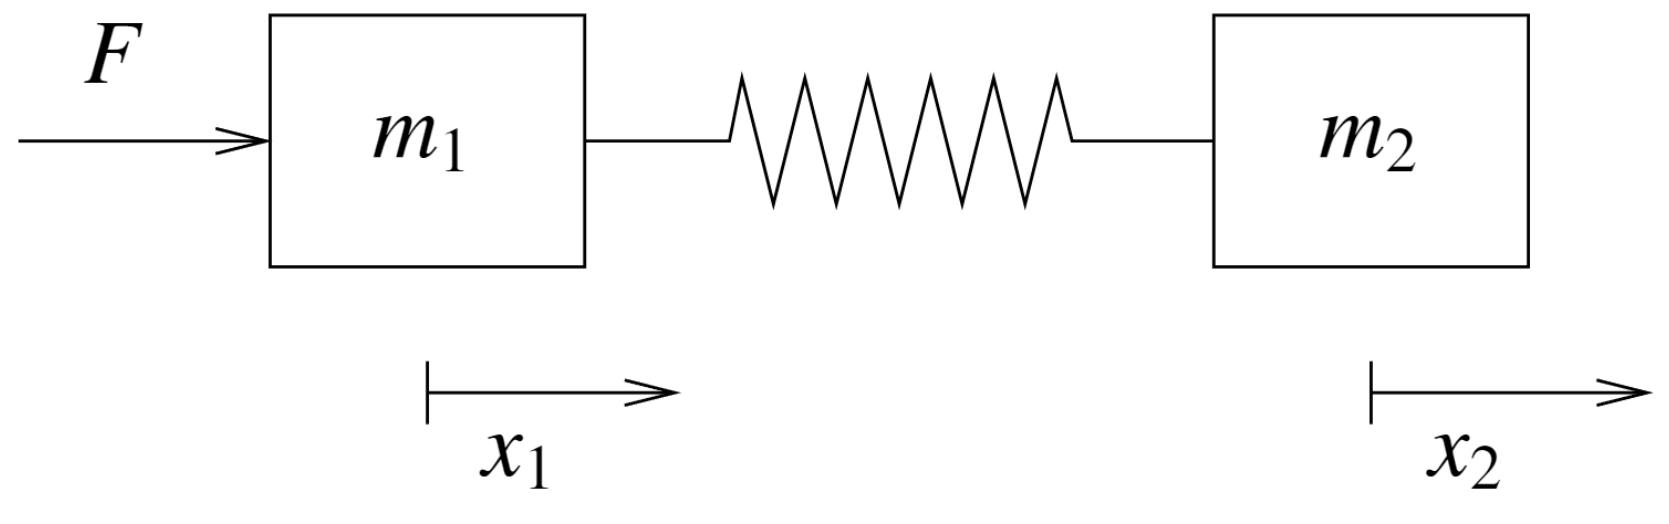
\includegraphics[width=0.5\textwidth]{two-cart-system.png}
\caption{Two cart system}
\label{fig:two-cart-system}
\end{figure}

\subsection{Non-Parametric Identification}
% [Report] For the non-parametric approach:
% 1) Frequencies/amplitudes used and why
% 2) Plots with magnitude/phase
% 3) Comparison with parametric identification

The non-parametric identification method used was sine-wave testing in conjunction with
the correlation method. This strategy consists of applying sinusoidal inputs at distinct frequencies
to calculate the magnitude and phase of the frequency response at that frequency from the correlation of
the time output of the system.

The frequencies used were 20 logarithmically spaced frequencies between 0.3 Hz and 10 Hz.
Too low of a frequency would not excite the system enough past the dry friction to get a good estimate of the
frequency response, while too high of a frequency would not be able to be accurately measured.
The amplitude chosen was 3V, which is a moderate amount of voltage to apply to the motor.
We experimented with different amplitudes; smaller voltages would not move the carts enough to overcome the static friction,
while larger voltages would cause the carts to drive off the railing. FIgure \ref{fig:bodeid_corr}
shows the Bode plot of the identified system using non-parametric identification.

\begin{figure}[!ht]
\centering
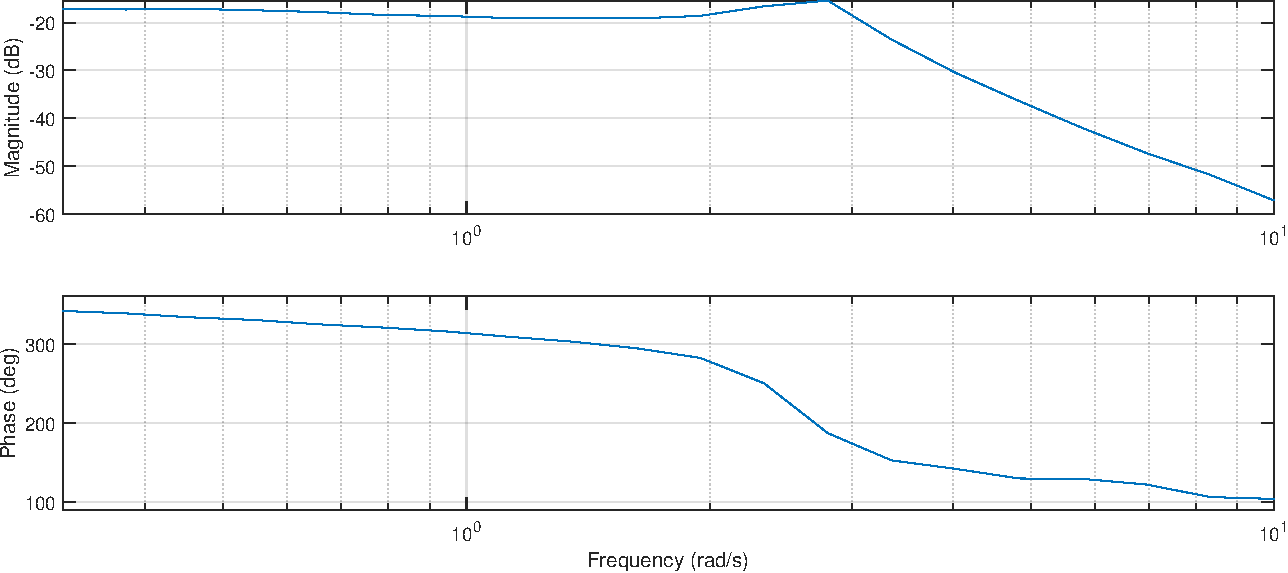
\includegraphics[width=\textwidth]{bodeid-corr.pdf}
\caption{Bode plot of the identified system using non-parametric identification}
\label{fig:bodeid_corr}
\end{figure}


\subsection{Parametric Identification}
% [Report] For the parametric approach:
% 1) Inputs used (square waves, chirp, etc.) and rationale
% 2) Plots showing input and output signals (representative examples)
% 3) Discussion of chosen model order, justification
% 4) Bode plots (magnitude and phase) of identified model
% 5) Comparison with non-parametric approach

In parametric identification, a constant number of poles and zeros are assumed in the transfer function.
Least-squares estimation is used to estimate the parameters of the transfer function given an experimentally obtained
set of time-domain input and output signals of the system.

The inputs used for the experiments were 20 sine waves with amplitude 3V and logarithmically spaced frequencies between 0.3 Hz and 10 Hz.
This was chosen to match the frequencies that worked well in the non-parametric identification method, and also to use the data obtained
from the non-parametric identification method to help estimate the parameters of the transfer function. A plot of the 20 outputs
obtained from the experiments is shown in Figure \ref{fig:outputs-param}.

\begin{figure}[!ht]
\centering
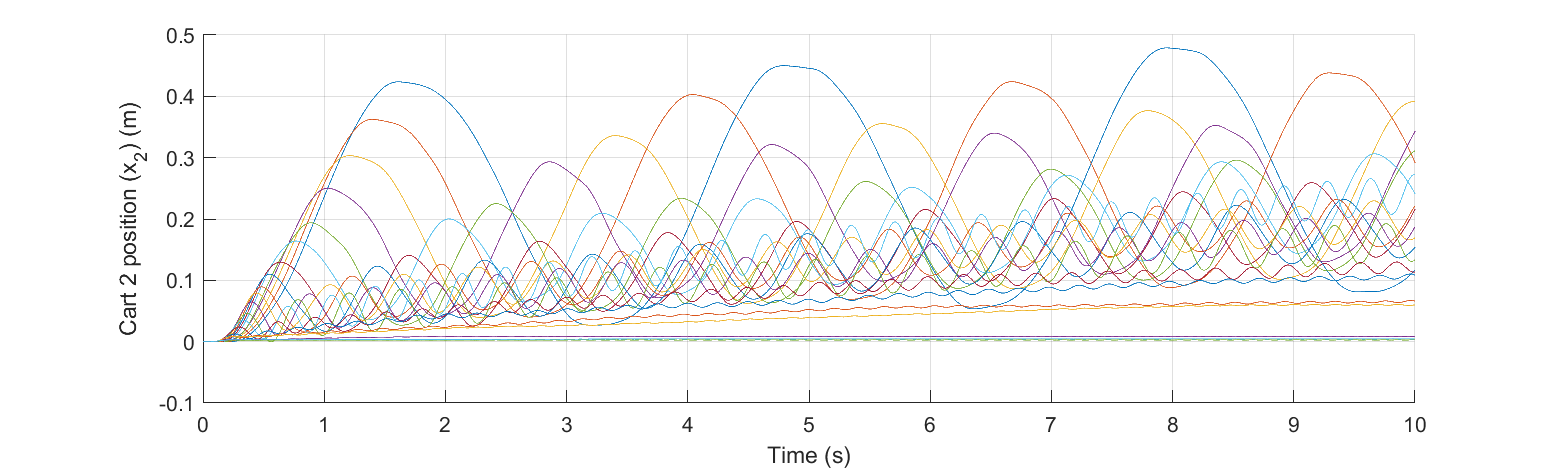
\includegraphics[width=\textwidth]{sysid-outputs.pdf}
\caption{Output signals of all experiments for parametric identification}
\label{fig:outputs-param}
\end{figure}

Least-squares estimation using the \verb|tfest| Matlab command was then performed for different numbers of
poles and zeros. The normalized mean square error (MSE) and the worst-case standard deviation of the parameters
were calculated for each model order, so the best model order could be chosen. These two metrics are shown in Figure \ref{fig:errors-param}.


\begin{figure}[!ht]
\centering
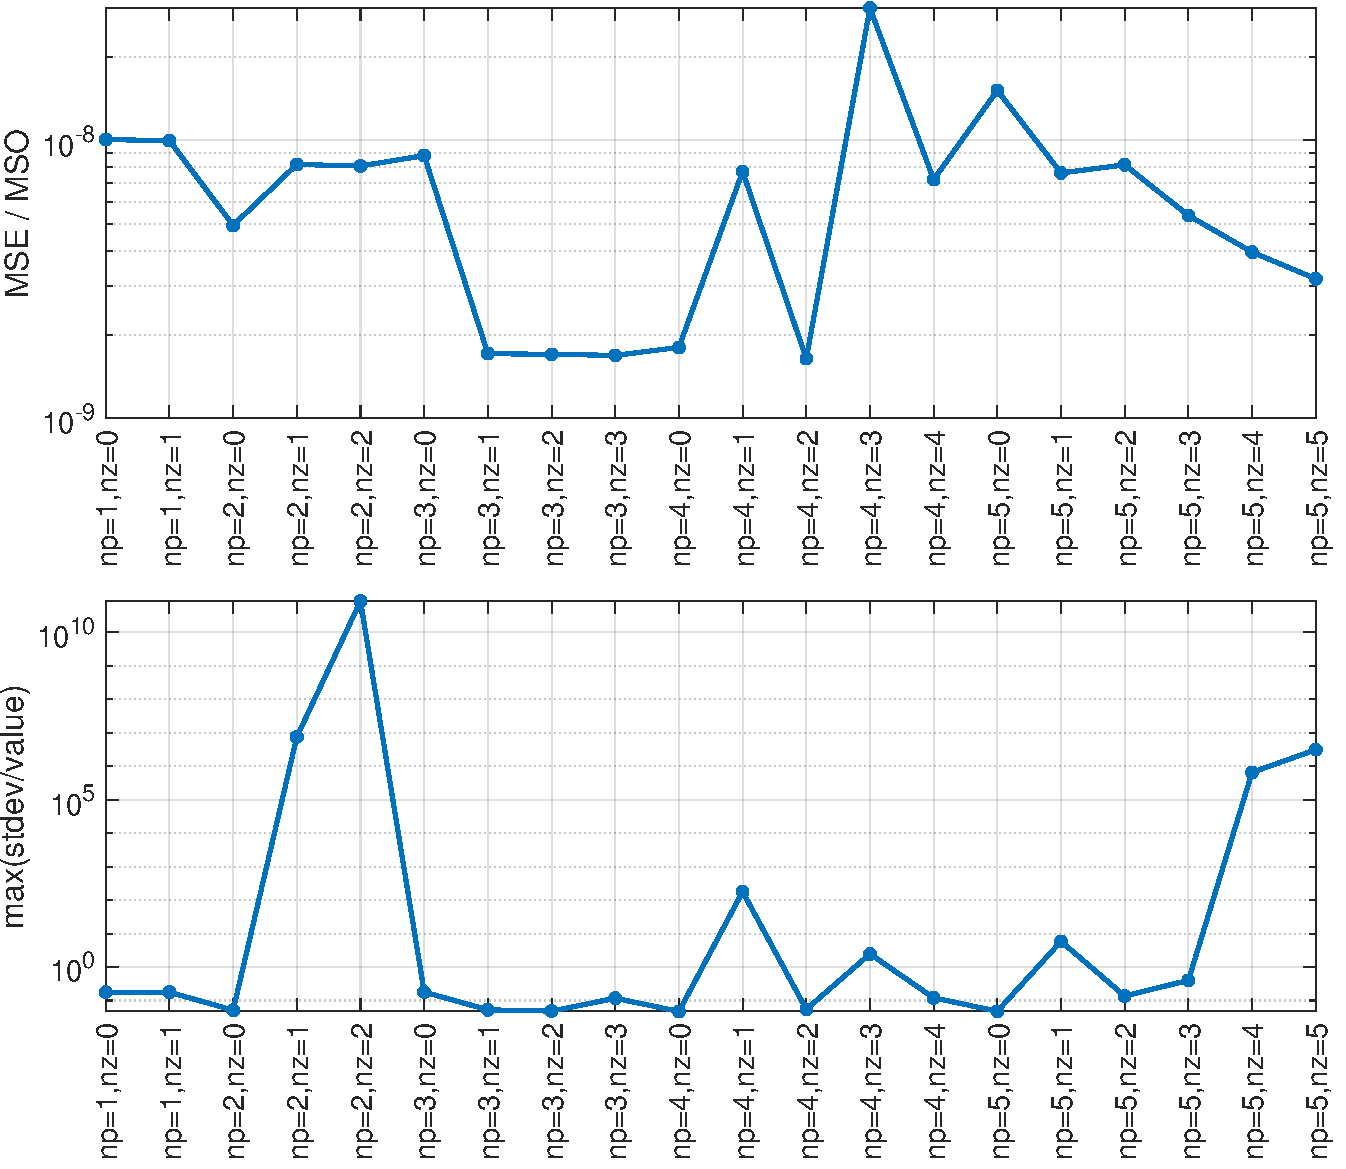
\includegraphics[width=\textwidth]{sysid-errors-fig.pdf}
\caption{Normalized MSE and worst parameter standard deviation for different model orders}
\label{fig:errors-param}
\end{figure}

Observing both plots in Figure \ref{fig:errors-param}, it can be seen that both metrics are minimized
for multiple different model orders. However, the choice of 3 poles and 2 zeros was chosen because it not only
minimized both metrics, but also produced the best Bode plot out of all of the estimated models.
The Bode plot of the identified system using parametric identification is shown in Figure \ref{fig:bodeid_param}


\begin{figure}[!ht]
\centering
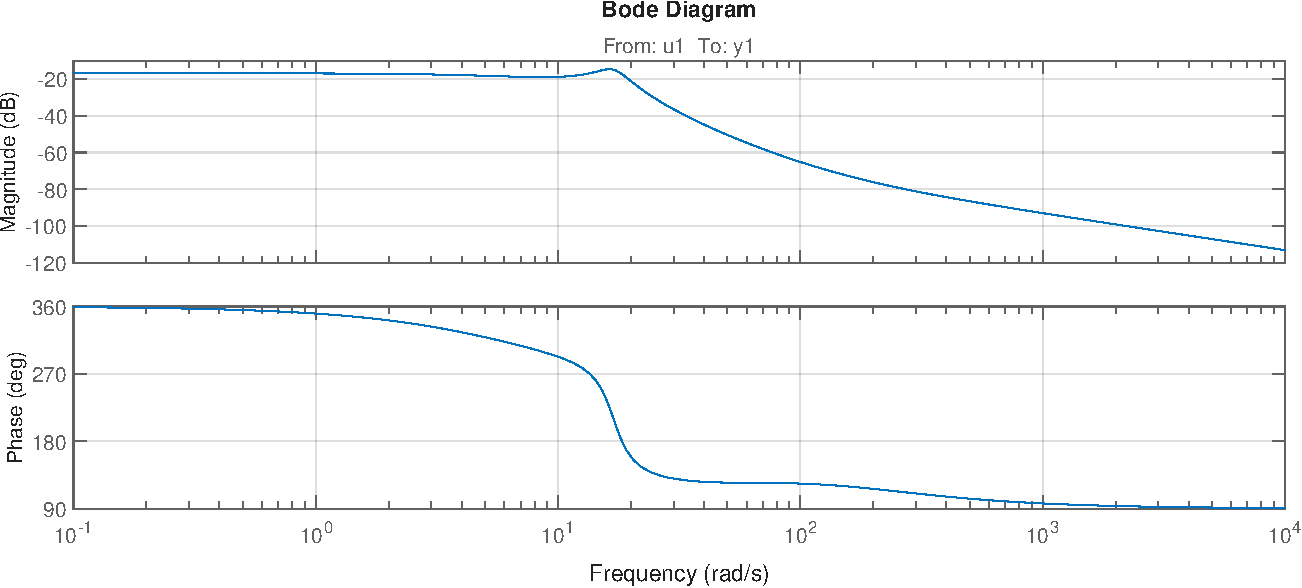
\includegraphics[width=\textwidth]{bodeid-param.pdf}
\caption{Bode plot of the identified system using parametric identification}
\label{fig:bodeid_param}
\end{figure}

\subsection{Comparison of Non-Parametric and Parametric Identification}

The results of the non-parametric identification method in Figure \ref{fig:bodeid_corr} and parametric identification method in Figure \ref{fig:bodeid_param}
are comparable in shape to each other. The non-parametric method has a higher gain at lower frequencies,
and its resonant frequency is also slightly higher. Also, with the non-parametric method,
the resolution of the Bode plot is limited to just the frequencies of the tested sine waves, but with
parametric identification, the resolution of the Bode plot is effectively infinite since it returns
an exact numerical transfer function.
However, all in all, both Bode plots look physically reasonable.
% ---------------------------------------------------
% 3. Controller Design
% ---------------------------------------------------
\clearpage
\section{Controller Design}
\label{sec:control}

\subsection{Design Methodology}

Next, we were tasked to design a controller for the system. We shot for an overshoot of less than 15\%
and a settling time of less than 2 seconds. To achieve this, we chose to use an LQR/LQG design. Using our 
identified model, we used Matlab to calculate the optimal LQR gains and Kalman filter. 

However, even with the optimal linear controller, the unmodelled dead zone of the motor still caused
there to be a large steady state error. To fix this, we added an integrator to the controller, which successfully
eliminated the steady state error. The final controller is an LQR/LQG controller in parallel with an integrator, which led
to a closed loop system with an adequate performance.

In order to combat integral windup and saturation of the motor, we added a 
clamping function to the integrator and controller output. This saturation
allowed us to achieve the limited steady state error of the integrator without 
suffering from the overshoot and instabilities that come from integral windup.
% [Report] Summarize the design approach:
% - Requirements (overshoot, settling time, etc.)
% - The control method chosen (PID, state-feedback, etc.)
% - Justification (why these gains, design trade-offs, etc.)
% - Possibly references to classical design or modern control design approaches

\subsection{Simulation Results}
% [Report] Provide:
% - Step response plots for the closed-loop system 
%   (using the identified model AND the nominal model from ECE147A&B, if relevant)
% - Bode plots for the closed-loop
% - Any relevant discussion about stability, noise, etc.
We simulated the closed-loop system in Simulink using the identified model. The frequency response
can be seen in Figure \ref{fig:bodecompsense}. The simulated step response is unstable, as 
seen in Figure \ref{fig:stepresponse}. However, as we will show, the controller still performs well in 
the actual system, as we tuned the parameters using the real setup in the lab.


\begin{figure}
\centering
    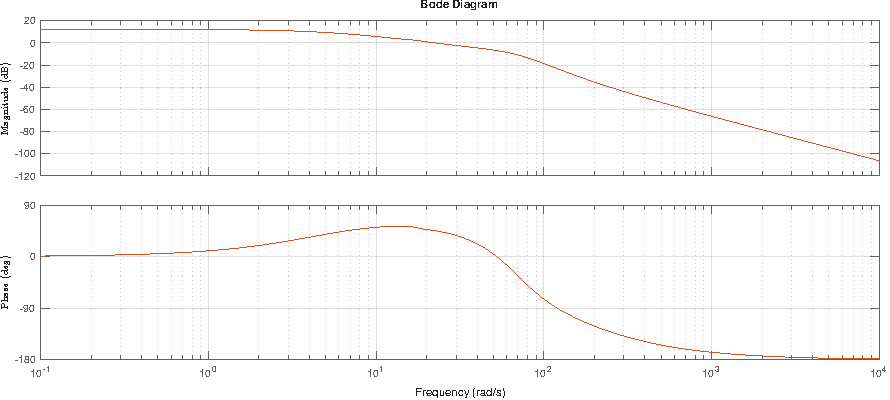
\includegraphics[width=0.7\textwidth]{bodecompsense.pdf}
    \caption{Closed-loop frequency response (simulated)}
    \label{fig:bodecompsense}
\end{figure}
\begin{figure}
\centering
    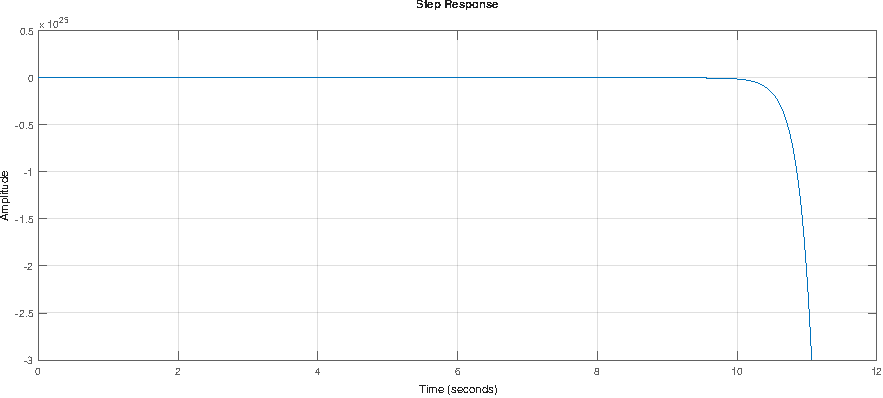
\includegraphics[width=0.7\textwidth]{bodecompsenseStep.pdf}
    \caption{Closed-loop step response (simulated)}
    \label{fig:stepresponse}
\end{figure}

% ---------------------------------------------------
% 4. Closed-loop Performance
% ---------------------------------------------------
\section{Closed-loop Testing}
\label{sec:closedLoop}

% [Report] Summarize the experiments performed in the lab with the actual hardware:
% 1) Step response data: include overshoot, rise time, settling time, max control input


% 2) Frequency response identification for the closed-loop (how you performed it, the results)
For the frequency response identification of the closed loop system, we ran a sinusoidal sweep across frequencies: $\omega \in 2 \pi [10^{-0.5},10]$
% 3) Discuss any discrepancies between theoretical and experimental results 
%    and possible reasons for them
The theoretical and experimental bode diagrams seem to disagree in phase and magnitude. This can be due to an inaccurate estimation of the order of the transfer function but ultimately we end up with a real closed loop that performs well so it is not too important.

\subsection{Step Response Experiments}
% [Report] Include a relevant plot/table with performance metrics (overshoot, rise time, etc.)
\begin{table}[h!]
    \centering
    \begin{tabular}{@{}lcc@{}}
    \toprule
    \textbf{Parameter} & \textbf{Value} \\
    \midrule
    Overshoot & 0.3\% \\
    Rise Time & 1.81 sec \\
    Settling Time & 2.23 sec \\
    Max Control Input &  5 V\\
    \bottomrule
    \end{tabular}
    \caption{Step Response Data}
    \label{tab:step_response}
\end{table}
    
% \begin{figure}[!ht]
% \centering
% 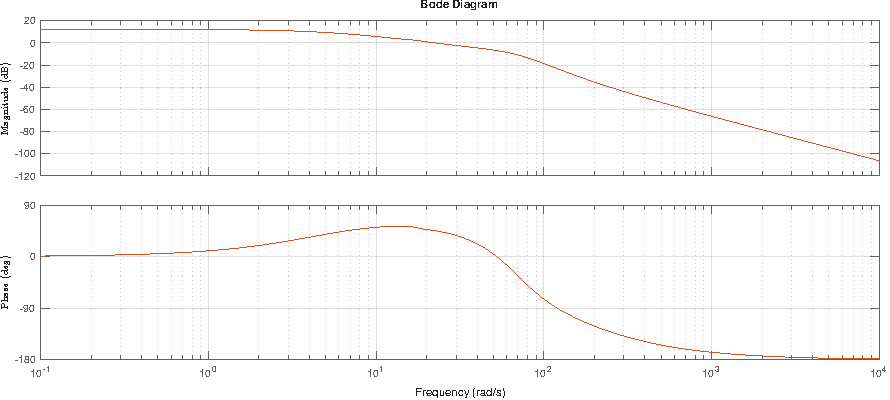
\includegraphics[width=\textwidth]{bodecompsense.pdf}
% \caption{Bode plot of complementary sensitivity function of simulated controller}
% \label{fig:bodecompsense}
% \end{figure}

% \begin{figure}[!ht]
% \centering
% 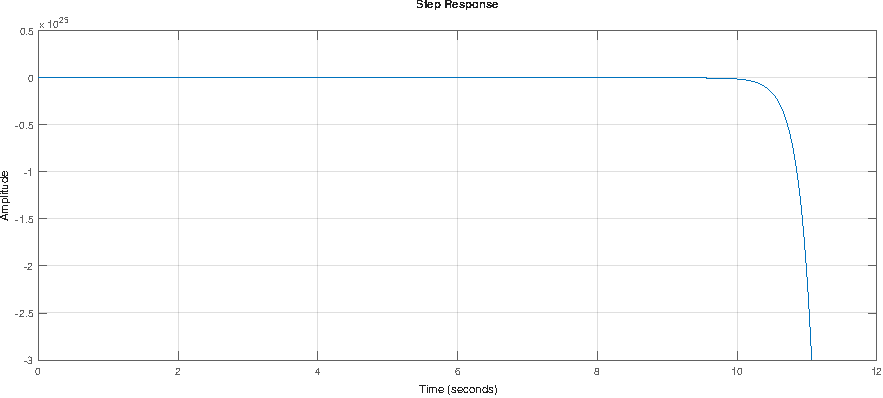
\includegraphics[width=\textwidth]{bodecompsenseStep.pdf}
% \caption{Simulated closed-loop step response}
% \label{fig:bodecompsenseStep}
% \end{figure}



\subsection{Closed-loop Frequency Response}
The closed-loop frequency response was identified using a sinusoidal sweep of the system. The results are shown in Figure \ref{fig:CLFreqResponse} and Figure \ref{fig:CLFreqResponseError}. The first figure shows the transfer function from reference to output, while the second figure shows the transfer function from reference to error.

\begin{figure}[!ht]
\centering
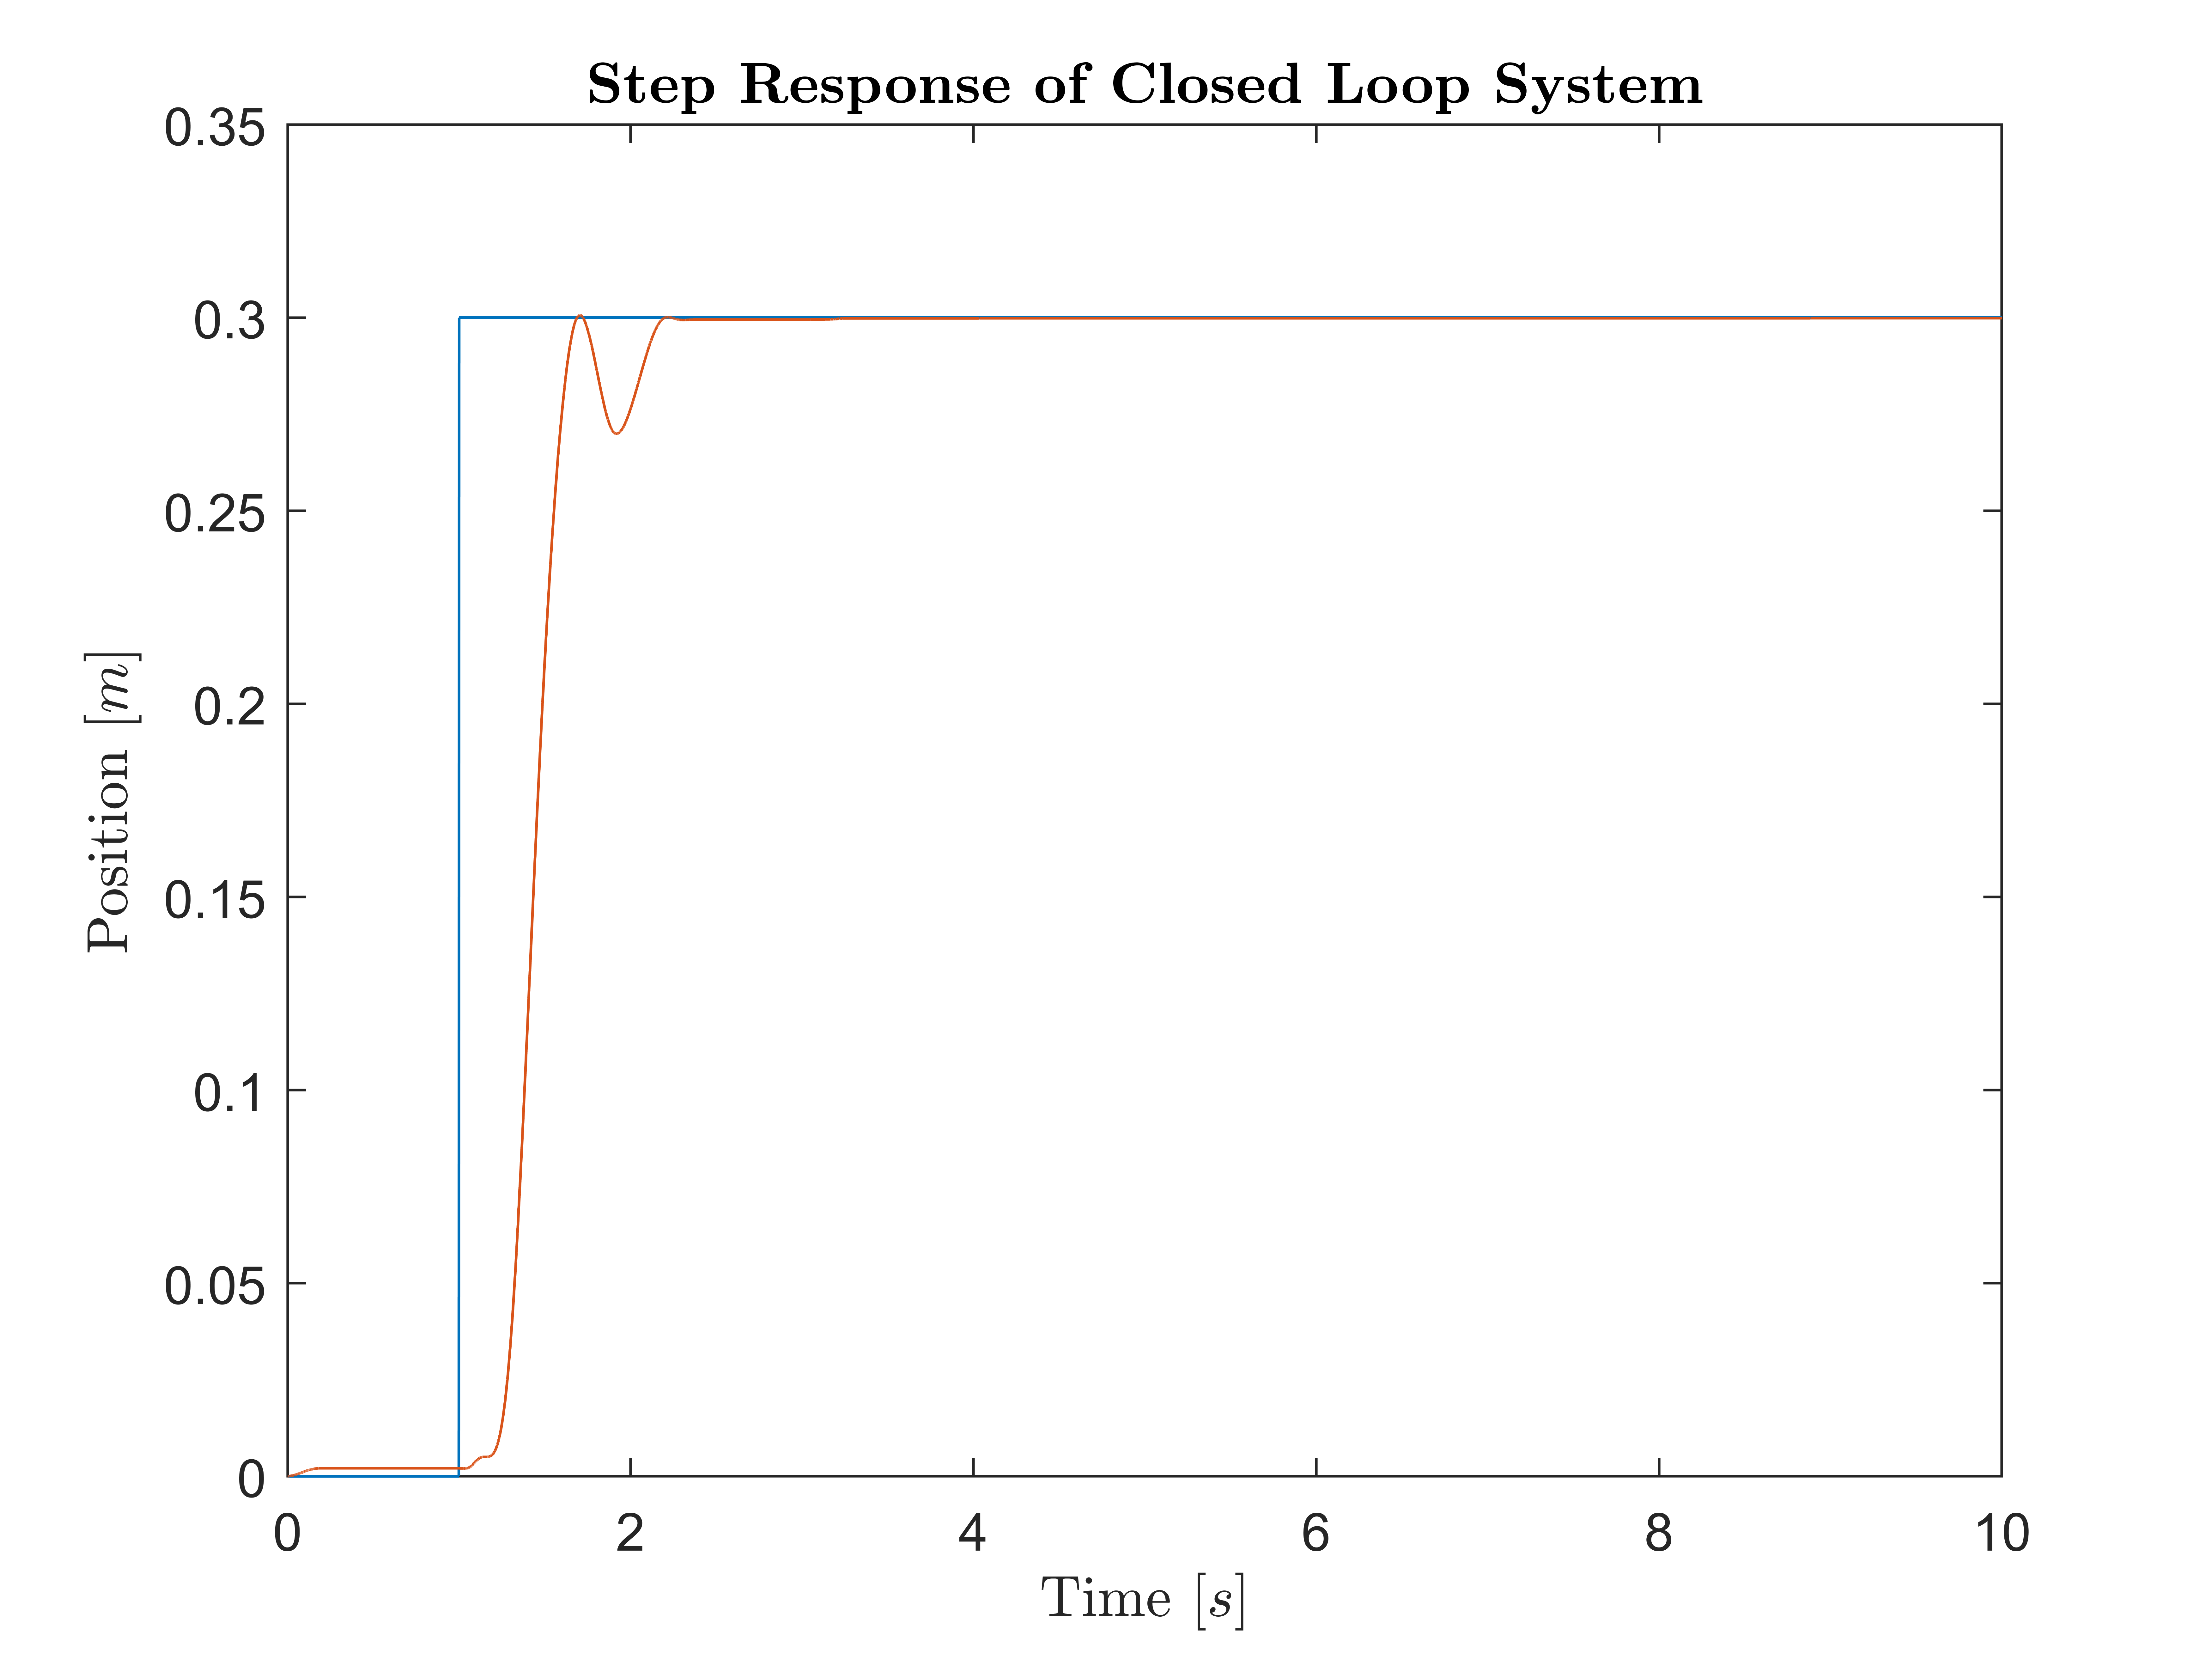
\includegraphics[width=0.7\textwidth]{CLStepResponse.png}
\caption{Closed-loop step response}
\label{fig:CLStepResponse}
\end{figure}


% [Report] Show how you identified the closed-loop frequency response
% (method used, plots, comparison with simulated predictions, etc.)



\begin{figure}[!ht]
\centering
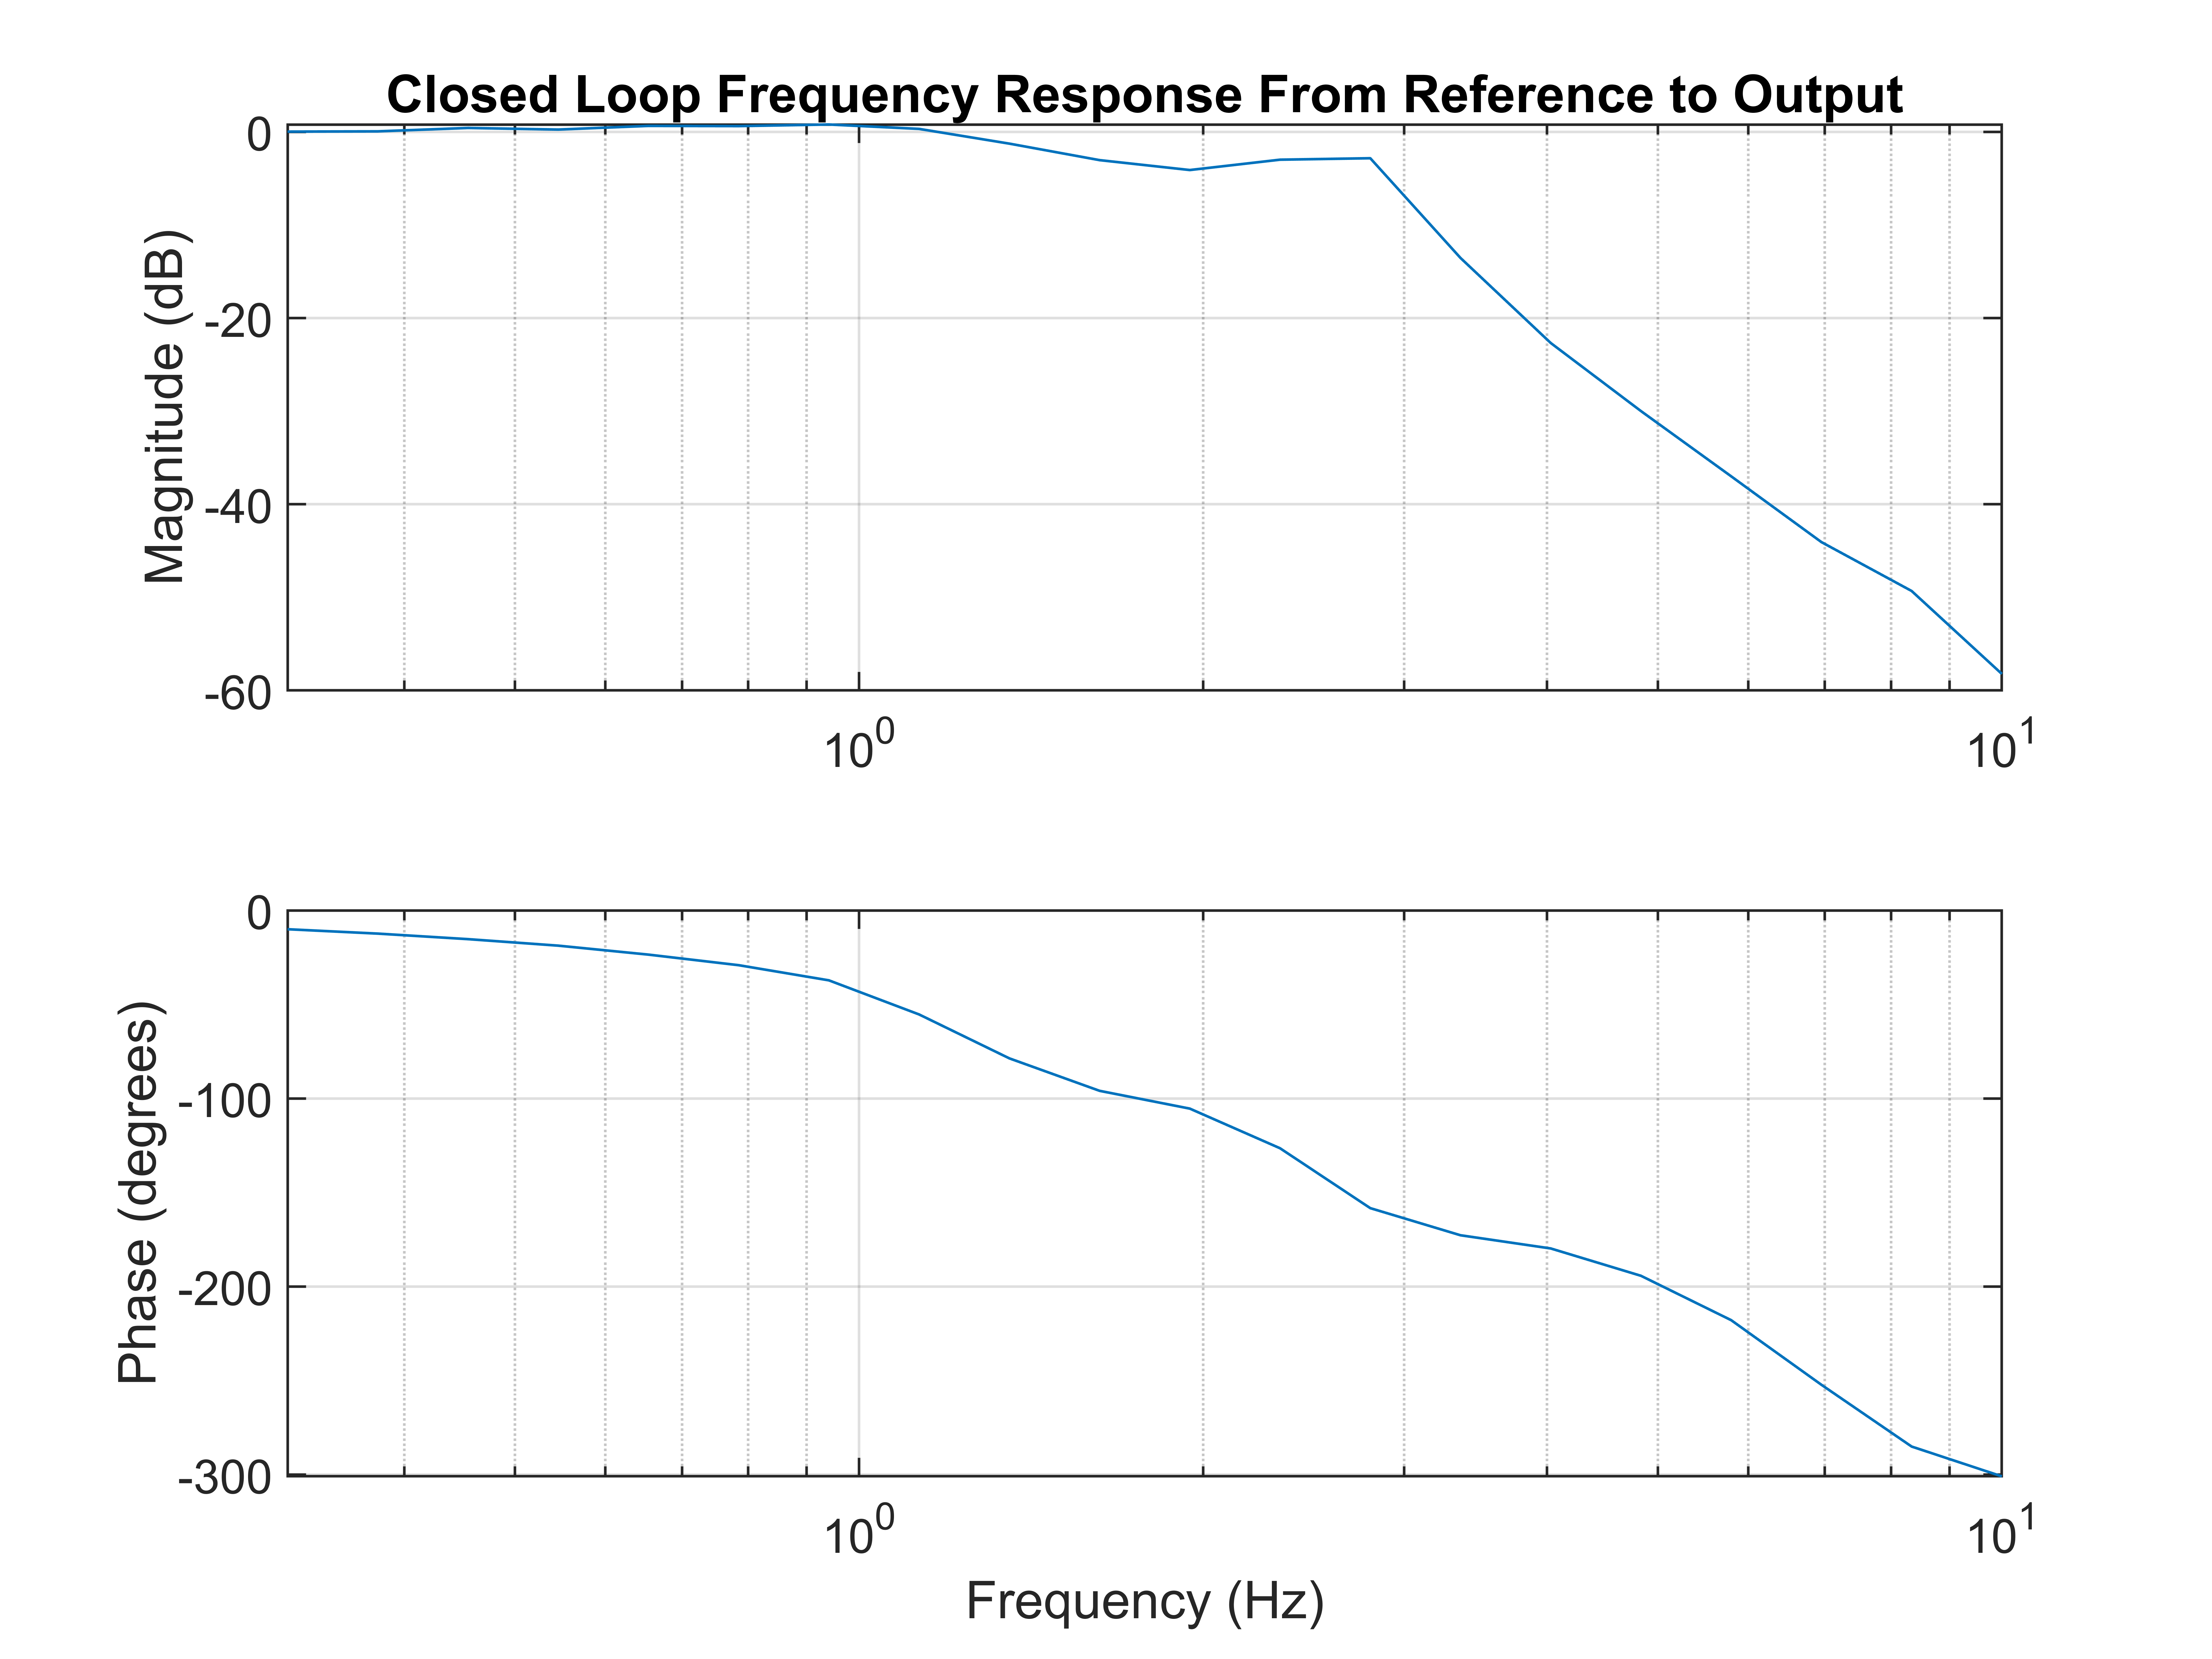
\includegraphics[width=\textwidth]{CLFreqResp.png}
\caption{Closed-loop frequency response of the transfer function from reference to output}
\label{fig:CLFreqResponse}
\end{figure}




\begin{figure}[!ht]
\centering
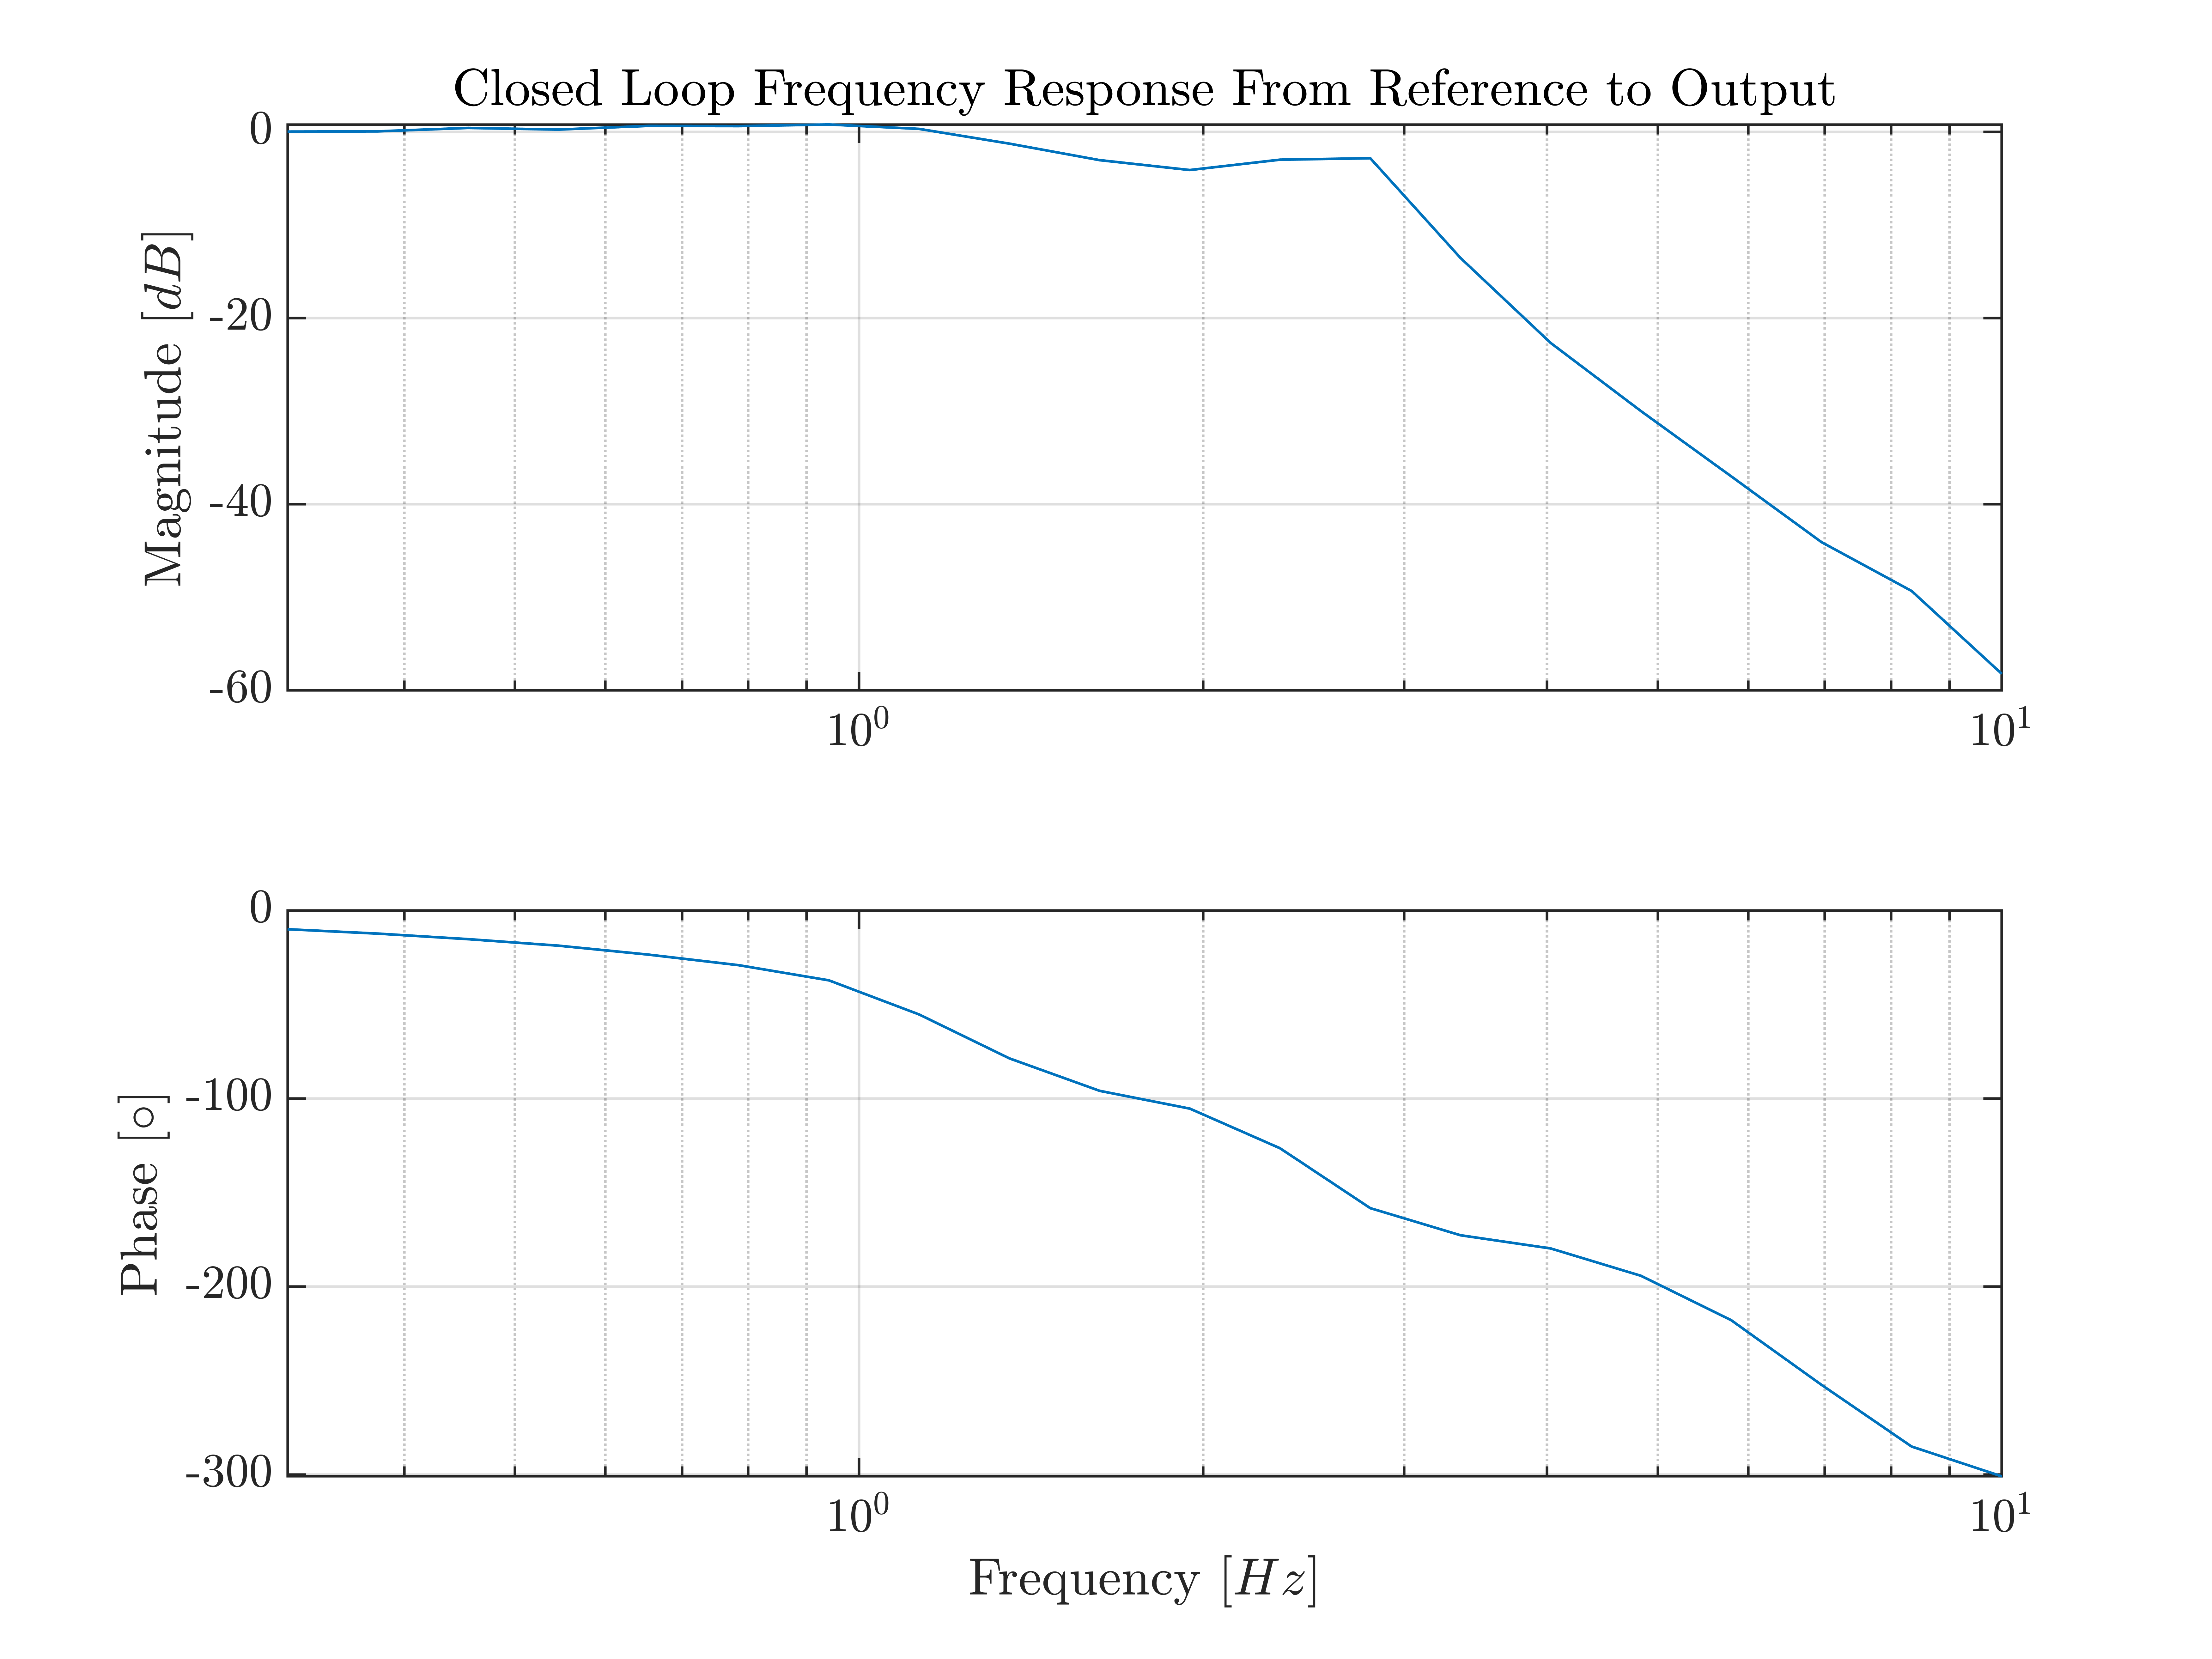
\includegraphics[width=\textwidth]{CLFreqRespError.png}
\caption{Closed-loop frequency response of the transfer function from reference to error}
\label{fig:CLFreqResponseError}
\end{figure}



% ---------------------------------------------------
% 5. Conclusions and Future Work
% ---------------------------------------------------
\section{Conclusions and Future Work}
% [Report] This normally covers:
% 1) Summary of main project achievements
% 2) Outline of what else could be done with more time or resources
We are happy with the performance of our controller and would love to improve it in the following ways. First, we ran a small sweep of frequencies but if we had more time, it may make sense to test many more frequencies with a finer mesh. Additionally, we could test a wider range to get better data about the noise and for higher frequency data. The sinusoidal sweep tests are simple, but it would also be interesting to try a test using a white noise input. 
Next, for the controller performance, we see that around resonance there is a large tracking error. This is a place which could use more work, but part of the issues could come from optimizing for that ideal step response behavior. 

% ---------------------------------------------------
% Reference

\end{document}
